\documentclass[conference]{IEEEtran}
\usepackage{cite}
\usepackage{amsmath,amssymb,amsfonts}
\usepackage{algorithmic}
\usepackage{graphicx}
\usepackage{textcomp}
\usepackage{xcolor}
\usepackage{fancyhdr}
\usepackage[hyphens]{url}

\newcommand{\arch}{ISER}

\newcommand{\shrink}{Eliminate vertical white-space}
\newcommand{\vshrink}[1]{
  \ifdefined\shrink 
	\vspace{-#1cm}
  \else
	\vspace{0cm}
  \fi
}

%\linespread{0.97}


\def\BibTeX{{\rm B\kern-.05em{\sc i\kern-.025em b}\kern-.08em
    T\kern-.1667em\lower.7ex\hbox{E}\kern-.125emX}}

% Ensure letter paper
\pdfpagewidth=8.5in
\pdfpageheight=11in

%%%%%%%%%%%---SETME-----%%%%%%%%%%%%%
\newcommand{\iscasubmissionnumber}{NaN}
%%%%%%%%%%%%%%%%%%%%%%%%%%%%%%%%%%%%

\fancypagestyle{firstpage}{
  \fancyhf{}
\renewcommand{\headrulewidth}{0pt}
  \fancyhead[C]{\normalsize{ISCA 2020 Submission
      \textbf{\#\iscasubmissionnumber} \\ Confidential Draft: DO NOT DISTRIBUTE}} 
  \fancyfoot[C]{\thepage}
}  

\pagenumbering{arabic}

%%%%%%%%%%%---SETME-----%%%%%%%%%%%%%
\title{\arch: Invisible Speculative Execution Through Data Recomputation} 
\author{}
%%%%%%%%%%%%%%%%%%%%%%%%%%%%%%%%%%%%

\begin{document}
\maketitle
\thispagestyle{firstpage}
\pagestyle{plain}

%%%%%% -- PAPER CONTENT STARTS-- %%%%%%%%

\begin{abstract}
\begin{verbatim}
    Brief problem statement: 
        Spectre, Meltdown, ++?
    Brief summary of recent arch. solutions: 
        Making speculative data invisible
    Proposed solution: 
        Recompute speculative load values
        Crisp description of high-level idea
        Pros, cons wrt related work
        Catchy evaluation numbers
\end{verbatim}

Recent architectural approaches to address speculative side-channel attacks aim to prevent software from detecting any changes %hide changes 
in the microarchitectural state while in speculation. 
%
%\emph{delay} changes until non-speculative, \emph{hide} changes and \emph{replay} when non-speculative, or \emph{cleanup} changes on mispeculation. In this work we focus on work that \emph{delays} changes until non-speculative.
One approach is to \emph{delay} micro-architectural changes until they are non-speculative. A \emph{Delay-on-miss} technique, simply delays loads that miss in the L1 until they become non-speculative, thus ensuring that transient changes in the memory hierarchy are not possible.
%
%To recover some of the latency, while waiting for the loads to become non-speculative, \emph{Value Prediction} (VP) of the delayed-load's value has been proposed.
However, this costs in performance and such techniques could not be improved unless a way is found to regain some of the delay. To this end, \emph{Value Prediction} (VP) of the delayed-load's value has been proposed as a solution.

%\textcolor{blue}{Too specific, sounds like fixing one particular problem, i.e., delay on miss and VP, instead of tackling the larger problem.}
In this paper, we show that the problem cannot be solved by simply introducing
%We observe that introducing 
a new kind of speculation (value prediction). 
Value predicted loads also have to be validated.
Waiting for the validation of these loads, results in similar occupancy of precious resources (hence similar stalls) as without the value prediction. Furthermore, validation serializes the execution of loads  \emph{even when such serialization is not imposed by the memory model}. The end result is that VP only yields marginal benefits over a baseline delay technique without VP.

%This has the unfortunate effect of \emph{serializing} validation of this speculation by seriof all loads that are value-predicted, \emph{even when such serialization is not imposed by the implementation of a memory model}. \emph{While loads that are value-predicted may contribute a little to ILP, their serialization detracts from MLP.} Because of this, the contribution of value prediction in the end performance is fundamentally limited.

Our insight is that we can achieve the same goal as value prediction (increasing ILP by early-performing some of the loads that miss) but without incurring its negative side-effect (serialization of validation and hindering of MLP) if we can \emph{non-speculatively} deliver load values on demand. 

We achieve this with \emph{Value Recomputation}, which trades computation for data transfer. This technique was previously proposed in an entirely different context: to reduce energy-expensive data transfers in the memory hierarchy. If we can safely, non-speculatively, recompute a value in isolation (without being seen from the outside), we do not expose any information that we would do otherwise, by transferring such value via the memory hierarchy.

In this paper we demonstrate the potential of recomputation in relation to a Delay-on-miss approach of hiding speculation and show that ... Results Results Results. Further, {\color{red} in contrast to VP where one pays a cost (energy, area) in hope of recovering some of the lost performance, recomputation is not only providing better performance than VP, but at the same time delivers its natural benefit which is an absolute reduction in data transfers in the memory hierarchy, hence an overall reduction in energy. This makes our proposal the first in which a more secure architecture surpasses the baseline in terms of energy-efficiency (EDP).
}{\color{blue} In the AMNESIAC paper, loads are never sent out to the memory system. In our work, we still need to access the L1, to determine if it is a miss or not.}





\end{abstract}

\section{Introduction}
\label{sec:intro}
\begin{verbatim}
    1 Problem statement: 
        Spectre, Meltdown, ++?
    2 Summary of recent arch. solutions
        Making speculative data invisible
        2.1 Overhead & complexity per se
        2.2 Limitations
        2.3 Coverage
    3 Proposed solution: 
        Recompute speculative load values
        3.1 Overhead & complexity 
            Put into perspective
        3.2 Limitations 
        3.3 Coverage
        3.4 Putting it all together:
            * Orthogonal to which, 
                alternative to what, ... wrt 2
            * Open new vulnerabilities?
\end{verbatim}


\section{Background}
\label{sec:back}
\subsection{Threat Model}
\label{sec:threat}
%\begin{verbatim}
  * Formal definition
  * Catchy motivating example?
 \end{verbatim} We do not need more sub-levels do we?
{ \color{red} [FIXME: Probably discuss after the shadows?] }

\subsection{Speculation Shadows} 
Sakalis et al. introduced the concept of \textbf{\emph{Speculative Shadows}} to reason about the earliest time an instruction becomes non-speculative and is considered safe to execute regardless of its effects on $\mu$-architectural state~\cite{sakalis2019efficient}.
%Instructions that can cast speculative shadows on younger instructions in the dynamic instruction stream are known as \textbf{speculation primitives}.
Speculative shadows can be of the following types: \emph{E-Shadows} are cast by any instruction that can cause an \textbf{exception}; 
\emph{C-Shadows} are cast by \textbf{control instructions}, such as branches and jumps, when either the branch condition or the target address are unknown or have been predicted but not yet verified; \emph{D-Shadows} are cast by potential \textbf{data dependencies} through stores with unresolved addresses (read-after-write dependencies); \emph{M-shadows} are cast by \textbf{speculatively executed memory accesses} that may be caught violating the ordering rules of a memory model (e.g., total store order---TSO) and therefore may need to be squashed; and \emph{V-shadows} that are cast by \textbf{value-predicted loads}~\cite{sakalis2019efficient}.

\subsection{Delay-on-Miss and Memory Consistency Models}
\label{sec:dom-vp}
%\input{dom-vp} We do not need more sub-levels do we?
The goal of Delay-on-miss is to hide speculative changes in the memory hierarchy (including DRAM). 
To achieve this, Delay-on-miss delays speculative loads that miss in the L1. Loads that hit in the L1 (and their dependent instructions) are allowed to execute speculatively as their effects (i.e., on the L1 replacement state) can be deferred for when the loads are cleared from any speculation shadow. 
The miss of a delayed load is allowed to be resolved in the memory hierarchy at the earliest point the load becomes non-speculative. An efficient mechanism to track shadows is proposed in~\cite{sakalis2019efficient}. 

A critical factor that affects the performance of Delay-on-miss (with respect to a non-delaying baseline) is its effect on MLP for the delayed misses. 
A stalled L1 miss is allowed to proceed (and affect changes in the $\mu$-architectural state) just after the \emph{first} load that caused the miss becomes non-speculative.
Many times, a single L1 miss satisfies multiple loads.\footnote{This property was exploited since the early high-performance architectures such as the Alpha 21164: each of its MSHRs could satisfy up to four outstanding loads that missed on the same cacheline~\cite{alpha21164}.} 
In such cases, MLP among loads to the same cacheline is attained effortlessly.
MLP, however, among loads on \emph{different} cachelines is more involved and depends on restrictions imposed by the memory consistency model (MCM). We will examine TSO and {\rc} as representative MCMs.

Assume that a delayed load exits all speculative shadows: E-Shadows (no instruction before it, or itself, will cause an exception), C-Shadow (all preceding branches have resolved), and D-Shadow (all preceding stores have resolved their addresses). The only shadow that is left is the M-Shadow that is governed by the MCM:
\squishlist
\item {\rc}: In {\rc} load$\rightarrow$load order is not enforced. An unperformed load does not cast an M-Shadow on younger loads, therefore there is no restriction on the MLP among delayed loads that are unshadowed.
\item TSO: In TSO load$\rightarrow$load order \emph{is} enforced and unperformed loads cast M-Shadows on younger loads, preventing them from releasing their L1 misses. However, even in this case there is a way to remove the M-Shadow. The key is non-speculative load-load reordering proposed by Ros et al.~\cite{aros-isca17}. Assuming that a load is unshadowed by any other shadow other than the M-Shadow, the M-Shadow can be removed by making the younger loads non-speculative via the cache protocol~\cite{aros-isca17}. \emph{Under this perspective TSO is no different than {\rc} with regards to Delay-on-miss MLP.}
\squishend

To conclude, one can argue that we do not need M-Shadows in any MCM: {\rc} does not have M-Shadows, and a TSO implementation that allows non-speculative load--load reordering~\cite{aros-isca17}, effectively eliminates the M-Shadows. 

Non-speculative load--load reordering delays remote stores which can be construed as a side-channel of a similar threat level to an invalidation side-channel~\cite{}. However, we stress here that this behavior is not a \emph{speculative} side channel as it only takes effect for \emph{unshadowed} loads, after they release their misses to the memory system.

\subsection{Delay-on-miss and Value Prediction} 

The concept of using value prediction with Delay-on-miss is to speed up the delayed loads (and their dependent instructions) and regain some of the lost performance. Unfortunately in our implementation VP, no mater how good we can make it (e.g., 100\% coverage and accuracy) gives only a limited benefit on tope of Delay-on-miss. VP cannot regain the lost performance. This is because of the following reason.

%VP needs to be validated. In order! Non-speculative load-load reordering cannot hep here as we are bound by a new speculation: VP-speculation (VP-Shadow). This prevents any MLP for the validation phase. Whatever VP wins in latency (pre-executing load and dependent instructions if correct), looses later in MLP. Result: limited.
In Delay-on-miss, the wast majority of all loads are executed speculatively (80+\% on average~\cite{}), which causes a notable fraction of the loads to be delayed. This takes up precious resources (i.e., the instruction queue, reorder buffer, load./store queue) and eventually stalls instructions from committing. Similar issues arise with other ``delay'' approaches such as NDA~\cite{} and STT~\cite{}.
The significant amount of speculation that is performed, results in each load being covered by several speculative shadows (five on average~\cite{}). This forces the majority of the loads to be executed serially, severely limiting MLP. Furthermore, removing any individual shadow (e.g., the M-Shadow) has a limited effect, as the load will be covered by another overlapping shadow.

VP cannot help much in this case, as it simply provides values early. The validation is still delayed until all shadows have been lifted. Thus, precious resources are still occupied until the same point in time as simply delaying.
The only perceptible difference is a faster commit of pre-executed dependent instructions if the validation of a value predicted load proves to be correct.

Furthermore, VP introduces a new speculative shadow, which we refer to as \emph{V-Shadow}. This new shadow is only lifted off from younger loads when the validation of the VP is complete. Thus, not only VP occupies precious resources in the same manner as the baseline Delay-on-miss, but further prevents younger loads from validating in parallel. The astute reader will note that this is the same as the M-Shadow an unperformed load casts on younger loads. Therefore a V-Shadow should not matter in the cases where we do have M-Shadows as the two shadows would completely overlap. As we argued above, we can eliminate the M-Shadow (even in MCMs that enforce load$\rightarrow$load ordering) which leaves the \emph{V-Shadow} as a liability that detracts from MLP and performance.
When VP coverage is fairly low, e.g., below 20\% as in~\cite{}, this effect is not pronounced, compared to the effect of removing the M-Shadow for all loads.

\subsection{Value Recomputation}
\label{sec:recmp}
%%%%%%%%%%%%%%%%%%%%%%%%%%%%%%%%%%%%%%%%%%%%%%%%%%%%%%%%%%%%%
\ignore{
--Both Spectre and Meltdown exploit speculative meta-data (generated by speculative loads).
--Target: Speculative code that makes *any* change in microarchitectural state, specifically cache hierarchy
    -- "Any futuristic attack caused by a speculative load" [InvisiSpec]
    -- What todo about stores?
    -- Does the type of load speculation matter? 
        --Mem consistency violation (depends on consistency model)
            -- A load reading data (i.e., being performed) before other loads or stores --preceding the load in program order-- are performed, may cause such violations...
        --Instr. at ROB head squashed (due to an exception e.g.), load was subsequent...
        --Branch misprediction (preceding branch)
        --St with address speculation; once address is calculated and matches a later load's (which already read data speculatively).
    -- We make speculation invisible in the data-cache, similar to InvisiSpec...
    -- We assume that everything operates correctly
%
    \begin{verbatim}
    Summarize Amnesiac
        [u-arch details go to main sect.]
    Put into perspective 
        "Security-aware" recomputation
        Cmp & Contrast
            Slice generation policy
        Vulnerabilities?
    \end{verbatim}
} We do not need more sub-levels do we?

{\color{red} To be completed by the Amnesiac team}

{\color{blue} Proposed as a way to trade in-core computation (cheap in energy) to data movement (expensive in energy) and at the same time perform better when the latency to re-compute is less than the latency to move data throughout the memory hierarchy.
\paragraph{Why RC can offer beyond VP}
Benefits in both latency and MLP: Latency: if recomputation is faster than a miss. MLP: No need to validate, hence does not impose any further restrictions on MLP, hence better performance. Energy: additional benefits in energy if recomputation needs less energy than data movement. Limitation: cannot do too much of it in practice. }

{\color{red} Magnus notes:
This can be observed for the case where an \emph{oracle} VP is used. One might think that a VP that has 100\% coverage and accuracy would perform equally to the recomputation oracle since the load value in both cases is provided immediately. But this is not the case. The vp-100 does not provide any significant improvement compared to the ISCA VP with ~20\% coverage (see nomralizedpc.pdf). For an improvement instant validation (no delay) is needed. VP is basically limited by the same "property" as delay-on-miss.

Recomputation alleviates this problem by removing the need to delay. A recomputed value is "instantly" (RC slice latency) available and can be committed as soon as all the shadows are lifted (in contrast to delay/VP, which requires a load/validation to be performed before commit).
}



 

\section{\arch}
\label{sec:arch}
\ignore{
\begin{verbatim}
 * Overview
    High-level exec. semantics
    Coverage wrt threat model
 * Detailed (micro)architecture
    * Buffers
    * ISA extensions
 * Putting it all together
    [Flowcharts?]
    * Behavior under speculation
    * Behavior under non-speculative exec.
    * Relation to value prediction
* Overheads?
* Correctness guarantee?
* New vulnerabilities?
 \end{verbatim}
 }
 
 \begin{figure*}
     \centering
     \subfloat[Slice example]{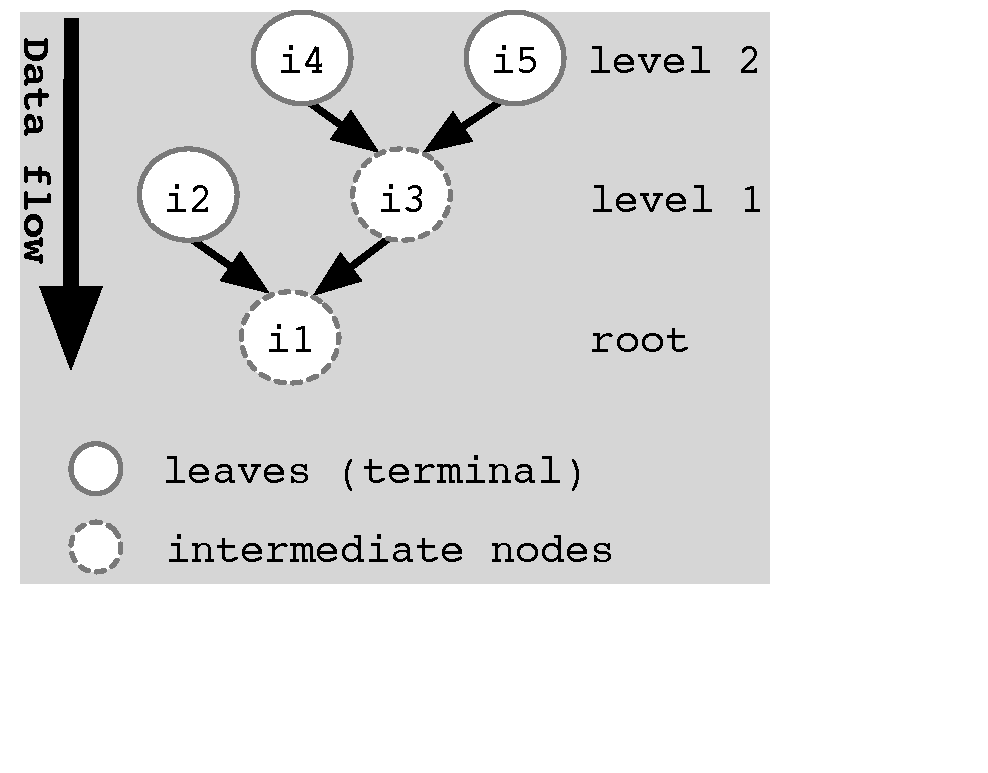
\includegraphics[width=0.3\textwidth]{figs/rt.pdf}\label{fig:rt}}
     ~~~
     \subfloat[Execution semantics and  $\mu$-architecture]{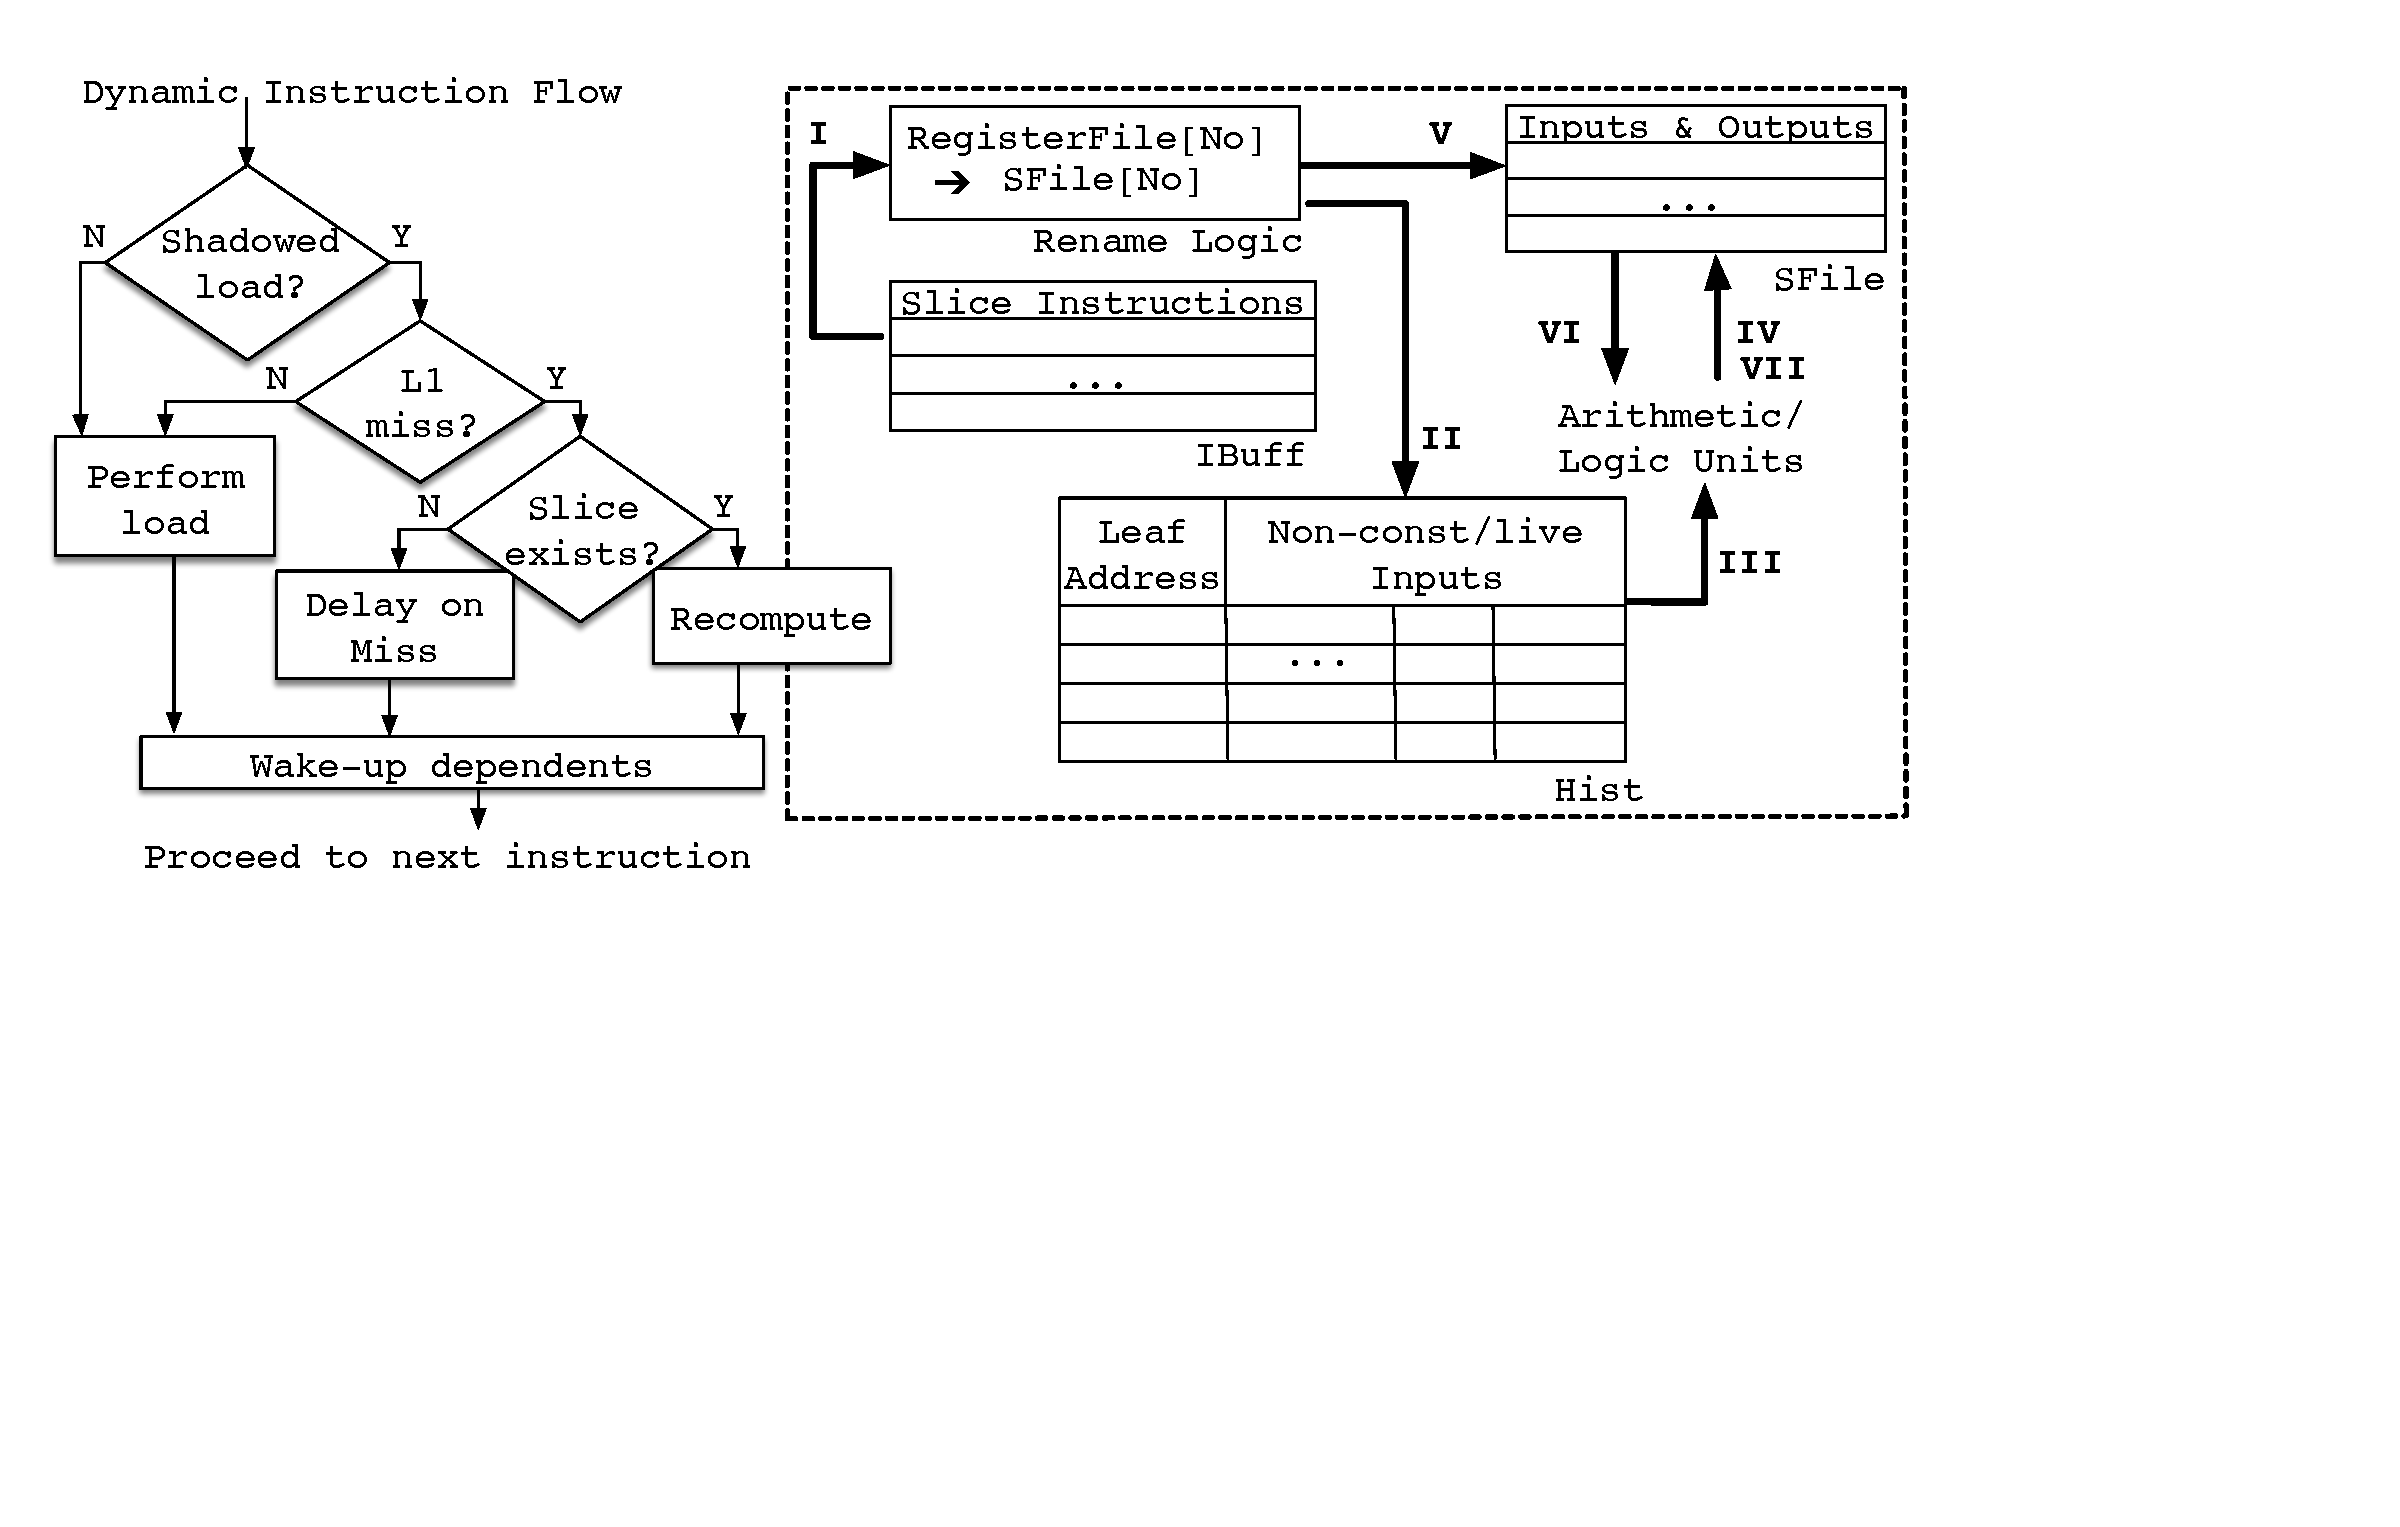
\includegraphics[width=0.57\textwidth]{figs/ctrl.pdf}\label{fig:ctrl}}
     \caption{ \arch\ Overview. All $\mu$-architectural buffers from (b) have  
an $\texttt{invalid}$ field per entry to
manage space (de)allocation.}
     \label{fig:overview}
\vshrink{.2}
\end{figure*}
 
% Overview
 
 \subsection{Execution Semantics}
 
 \arch{} only resorts to recomputation to regenerate values that otherwise would be read by a speculative load from the memory hierarchy, and only so, if the respective speculative load misses in the L1 cache. Recomputation takes place as long as a slice exists and the input operands to the slice instructions can be made readily available (see \autoref{sec:slice_formation} on slice formation).
 %This execution model has the potential of delivering higher energy efficiency, as imbalanced technology scaling renders loads much more energy hungry and slower than arithmetic/logic instructions (which form slices)~\cite{Horow}. 
 %Typically a slice contains \redHL{no more than 10-15 instructions}.
 
\ignore{
Not all of the input operands of leaf instructions of a slice can be
(re)generated by recomputation.  This may be the case if input operands
correspond to (i)~read-only values to be loaded from memory, such as program
inputs; or (ii)~register values that are lost, i.e., overwritten at the time of
recomputation. We will refer to such input operands as {\em non-recomputable}
inputs. For \recomp\ to work, non-recomputable inputs of slice-leaves
should not only be available at the anticipated time of recomputation, but also
be retrievable in an energy-efficient manner.
%
%Recomputation cannot eliminate any memory access to retrieve the non-recomputable inputs of slice leaves.  
If non-recomputable inputs do not
reside in close physical proximity to the processor, the energy cost of their
retrieval may easily exceed the energy cost of memory accesses, rendering recomputation useless.    
Buffering can help in this case. No dedicated buffering is necessary if the leaf input operands
correspond to constants or live register values. 
}

While \arch\ shares basic microrachitectural structures with Amnesiac~\cite{amnesiac17} to facilitate \recomp\ (such as dedicated buffers to prevent corruption of $\mu$-architectural state during recomputation), its
execution semantics are quite different when it comes to slice identification and triggering recomputation.
%, and committing recomputed values to architectural state. 
These stem from the defining difference in optimization targets: Amnesiac uses \recomp\ to maximize energy efficiency irrespective of security implications. \arch, on the other hand, uses \recomp\ to eliminate (already known or yet to be discovered) threats induced by speculative loads. 
In a nutshell, differences between Amnesiac and \arch\ expand along two axes:
%Putting it all together, execution semantics are different than Amnesiac~\cite{amnesiac17} in the following ways:
 \begin{itemize}
     \item{\em What to recompute (slice identification):} As opposed to Amnesiac, \arch\ does not impose any direct constraint 
     %on slice length 
     to preserve energy efficiency,  as we are not after minimizing energy or latency per load. As long as a slice exists, and its inputs can be made readily available at the anticipated time of recomputation, \arch\ would consider it for recomputation. The only practical limitation on slice length may stem from storage overhead of $\mu$-architectural buffers in this case. 
     \item {\em When to recompute:} \arch\ swaps speculative loads that miss in L1 for recomputation (i.e., with producer instructions of the respective value along a slice). Amnesiac on the other hand, triggers recomputation (irrespective of whether the load is speculative or not) only if it is more energy-efficient to do so. 
 %    \item{\em How to recompute?} Similar to Amnesiac, we use dedicated buffers to prevent corruption of $\mu$-architectural state. 
     \ignore{
     \item{\em When/how to commit a recomputed value to architectural state:}
     \textcolor{blue}{\\ HMS: {\recomp} is non-speculative and safe, they don't have to adhere to the shadows. It's the action of the load itself that has to be avoided, which it is, so the {\recomp} computed value can be treated as any other transient register, e.g., the result of an addition. Thus, I don't see any difference compared to Amnesiac. 
     U: Noted, and elimiated\\}
     In Amnesiac, a recomputed value is written into the destination register of the  load before execution resumes from where the corresponding load (which is swapped for recomputing instructions) has left. 
     \arch\ has to keep these values buffered until the speculation is resolved (i.e., all shadows are lifted).  
     \recomp\ cannot change architectural state under speculation, by definition. {However, just as speculative loads that \emph{hit} in the L1, recomputed loads pass their value (in a physical register) to dependent instructions and advance execution.} }
 \end{itemize}
 
 In the following sections, we will cover design specifics, limitations, and side effects of \arch, with a special focus on coherence and consistency implications. 
 
% We will detail design specifics next. 
 
\subsection{Slice Formation \& Annotation}
\label{sec:slice_formation}

%\noindent{\bf Slice Formation:}
Similar to Amnesiac, we rely on a compiler pass (backed up by profiling) to form and annotate slices, which 
 mainly constitutes
%first estimates,
%probabilistically 
%(as detailed in the following and Section~\ref{sec:setup}),
%\footnote{Section~\ref{sec:setup} details a representative
%probabilistic model based on memory access statistics collected from profiling.}
%the energy
%consumption of loading $v$, $E_{ld,v}$. Next comes 
%with 
dependency analysis to
identify the producer instructions for each load.\footnote{Instead of a compiler,
%, in order to calculate the anticipated
%cost of potential recomputation.
%\textcolor{blue}{HMS: I think this idea is currently too immature to be included.}
%\redHL{U: Our implementation is actually Pin-based, if this is what you were referring to?}
%\textcolor{blue}{HMS: I might have misunderstod the text. I was reading the following text as it could be done at runtime while executing the application (in deployment every time the application is run), not as a "profiling pass".}
%\redHL{Yes, this may open Pandora's box, need to clarify.}
%{\color{magenta}  
the same job can be performed by \emph{dynamic binary instrumentation} at run time (albeit with probably inferior alias analysis but more dynamic information), rendering recompilation unnecessary in deployments where it is not an option.}
Slice creation is a \emph{best effort} under strict validity guarantees. Not being able to generate a recomputation slice for a load is not a security weakness under a security technique such as Delay-on-Miss, but simply a missed optimization opportunity.
 Although in this paper the slice formation is conservative, as we will see later, the requirement for strict guarantees of the recomputation validity can be relaxed (potentially increasing the coverage of recomputation, i.e., portion of load values that can be recomputed, and addressing coherence issues) if the appropriate architectural support is available. However, such extensions are outside the scope of this paper and will be fully evaluated in future work.
%}

The slice formation pass builds the slice as a data-dependency graph, where
%%This step starts building the slice (where 
the immediate producer of the value to be loaded resides at the root (Figure~\ref{fig:rt}).
%%), and lets the slice grow
%%level by level. 
As opposed to Amnesiac, the restriction to slice length comes from slice inputs or storage requirements (rather than the associated energy cost). 
%, as long as the cumulative cost of recomputation along \rsv\
%being constructed remains below $E_{ld,v}$.     
If, during the traversal of data dependencies, we encounter other load instructions, we 
%As the compiler traverses the dependency chains, it may hit
%load instructions. In the proof-of-concept implementation, the
%compiler replaces each such load 
replace them recursively with the respective producer instructions. 
%recursively.
This recursive growth can continue until a store to the same address is encountered.
Loads and stores cannot be present 
%as intermediate nodes 
in any slice by definition.
%In fact, stores can never find place in \rsv, and loads can only, if at all,
%appear at the leaves to read non-recomputable input operands.

Once construction is complete, 
%corresponding 
each slice gets embedded into the binary. 
Similar to Amnesiac, the special control
flow instruction $\texttt{RCMP}$ communicates recomputation opportunities to the runtime, which
%we use 
%\noindent {\bf Slice Annotation:}
%\label{sec:isa}
%As a hint for the runtime scheduler, the compiler replaces each load that has a slice
%the swap
%of which with recomputation is likely to be more energy-efficient (according to
%the probabilistic energy cost comparison explained above) 
%with a 
semantically corresponds to an atomic bundle of a conditional branch + load (where no prediction is involved for the ``branch'' portion).
%In this manner, the recomputing instance of an
%instruction is separated from its original, ``computing'' instance.
%Semantically, $\texttt{RCMP}$ corresponds to the fusion of a conditional branch
%with a load\footnote{
%Depending on the specifics of the underlying instruction set architecture (ISA),
%$\texttt{RCMP}$ can also be synthesized by a pair of branch and load
%instructions, without loss of generality. 
%}. 
The runtime scheduler resolves the branching condition: if the respective load (while shadowed) misses in L1, $\texttt{RCMP}$ acts as a jump to the entry point (starting from the
terminal instructions) of the corresponding slice. Otherwise (i.e., if the load hits in L1 when shadowed or if the load is not shadowed), $\texttt{RCMP}$ acts as %is not any different than 
a classic load.
All operands of the respective load and the starting address of its slice form the operands of the $\texttt{RCMP}$. 
%During runtime we can re-order the leaf instructions in a slice, as leaf instructions cannot depend on each other. 
An $\texttt{RTN}$ instruction (similar to a procedure return in nature) demarcates the end of each slice and returns the control to the instruction following the $\texttt{RCMP}$. Before the return takes place, the recomputed value is provided to the consumers of the respective load, in the same way as if the load was actually performed (i.e., by passing the value in a physical register). 
%\recomp\ cannot change architectural state under speculation, by definition. However, just as speculative loads that \emph{hit} in the L1, recomputed loads pass their value (in a physical register) to dependent instructions and advance execution.
%However, the destination register of the corresponding load only gets updated after the load becomes non-speculative.


%\ignore{
As explained by Akturk and Karpuzcu in~\cite{amnesiac17}, recomputation is possible, even if the compiler cannot prove that all input operands of
terminal instructions correspond to immediate or live register values at the anticipated
time of recomputation, by keeping such input operands (e.g., overwritten register values) in a dedicated buffer.
For any operand of this sort a $\texttt{REC}$
instruction is inserted directly after the instruction producing the value of the operand.
%Only if slice leaves have operands of this sort, $\texttt{REC}$ instructions find place in the binary.
%, which serve buffering of the respective input operands such as
%overwritten register values.
%as detailed in Sections~\ref{sec:micro} and~\ref{sec:sched}.  
%An $\texttt{SLC}$ instruction
%goes right before the entry point of \rsv.  $\texttt{SLC}$ has a single integer
%operand, $\texttt{RSlice-ID}$ to carry the unique ID of \rsv.  
%
%An $\texttt{REC}$ instruction follows each instruction, a replica of which represents a leaf in the slice. 
$\texttt{REC}$ takes as operands the destination register of the previous instruction and an
%two 
% a single 
integer operand:
%$\texttt{RSlice-ID}$, and 
$\texttt{leaf-address}$, which points to the address of
the corresponding terminal instruction in the slice.  
$\texttt{REC}$ practically checkpoints the input
operand 
%of its predecessor (which form the non-recomputable inputs
%of the leaf at $\texttt{leaf-address}$) 
to a dedicated buffer. 
%}
%{\color{magenta} The target address of the producer instruction (e.g., store) is also saved as a tag for the whole slice in this dedicated buffer. This tag can be matched by future stores on the same address, to invalidate the slice (and cancel recomputation).}

\subsection{\arch{} Architecture}
\label{sec:iser-architecture}

\arch{} implements the shadow tracking technique proposed by Sakalis et al.~\cite{sakalis+:ISCA2019vp}. %
The shadow tracking consists of a \textit{shadow buffer} (SB) that acts as a circular buffer similar to the reorder buffer (ROB). %
When a shadow casting instruction enters the ROB a new entry is allocated at the tail of the SB. %
Every load that enters the ROB checks the SB and if not empty, an entry is allocated in a \textit{release queue} that associates the load with the youngest entry in the SB (i.e., its tail). %
The load remains speculative as long as the head of the SB is marked as unresolved and not equal to the SB entry associated with the load. %
This mechanism performs a simple comparison between the head of the release queue and the head of the shadow buffer to identify when loads exit all their shadows,
thus, avoiding the need for costly content addressable memory~(CAM) searches. %


We detail next the $\mu$-architectural structures depicted in Figure~\ref{fig:ctrl}, which serve two main purposes:
(1) Keeping $\mu$-architectural state intact during recomputation; 
(2) Making slice instructions and operands available at the time of recomputation.

\ignore{
Figure~\ref{fig:ctrl} depicts microarchitectural support to meet  {
Condition-I} and {Condition-II} in orchestrating recomputation.  Recall
that, for simplicity, only one slice can be active, i.e., traversed for recomputation, at a
time but that can be rectified with a more elaborate $\mu$-architecture. 
%{\color{red} STEFANOS: I don't understand this restriction. We're just injecting more instructions in the instruction queue. If we encounter another load that can be recomputed we insert more instructions in the IQ and let everything run at max ILP. In other words I do not see the reason why we do not allow RLP (Recompute-Level-Parallelism). Maybe because the call-return semantics of recomputation? Bur even so, we can execute functions in parallel by predicting  their returns!}
%\footnote{Offloading recomputation to spare or idle cores, or using helper threads may improve energy efficiency further by enabling concurrent recomputation. However, the basic proof-of-concept implementation assumes strictly sequential execution semantics.}
%ULYA: Ack. This is coming from our previous analysis which we didn't consider OoO execution in detail. But at the same time, I'd sparee detailed discussion of this for now (unless we want to get deep into microarchitecture here). 
}

\noindent {\em The Scratch-File (SFile)}  practically acts as the physical register file during recomputation. 
Specifically, while recomputation is in progress, all data flows through the SFile. Thereby, \arch\ preserves $\mu$-architectural state during recomputation. No structure beyond SFile is necessary in this case, as no memory access instruction is permitted in a slice.

\noindent {\em The Rename logic} translates (architectural) register references of slice instructions to SFile entries.
Semantically, it is equivalent to the rename logic of classic out-of-order processors, with SFile replacing the physical register file. 
%\textcolor{blue}{HMS: How are registers stored in the Hist buffer referenced, i.e., how can an instruction specify if the value is to be read from an architectural register, the SFile, or from a value in the Hist that has been stored by an REC instruction?}
%\redHL{U: It is the recomputation pipeline from Fig.1b, please check updated text. Recomputing instructions always have their data supplied from this pipe, even though they share exec. units with the rest of instructions. Here is more detail from ASPLOS paper (which we can include here): We need to differentiate between leaves and intermediate nodes, since different structures supply the input source operands to each: The inputs of leaves can come
%from the register file (a live value) or Hist (an overwritten value). The inputs of intermediate nodes come from
%SFile. The compiler can annotate leaves and accesses to Hist
%to distinguish between these cases. Specifically, the compiler can change source register identifiers of leaf instructions
%reading their operands from Hist to an invalid number. Leaf
%instructions with valid source register identifiers directly access the register file.}
%\textcolor{blue}{HMS: The paper gives the impression that only three new isntructions are needed RCMP, RTN, and REC but wouldn't this require more or less a duplication of many of the instruction set as the instructions have to be able to distinguish between if they are leaves or not and between register file or hist?}
%\redHL{Not necessarily, as the above text suggests we can play with special operand codes.}

\noindent{\em  The Instruction Buffer (IBuff)}
%The dedicated instruction buffer IBuff 
caches slice instructions in order to avoid
%within each slice, in order to relax {\color{red} ISER} amnesic execution's 
unnecessary pressure on the instruction cache.
Each entry of IBuff corresponds to a recomputing instruction. Fetch logic fills IBuff, similar to the instruction cache. IBuff feeds the rename logic. 
%once the traversal of (i.e, recomputation along) an \rs\ finishes.  

%\ignore{
\noindent {\em The History Table (Hist):} 
For each slice  where the input operands of terminal instructions represent immediate or live
 register values, no additional buffering is necessary.
 Otherwise,  
 %{Condition-II} is automatically
%satisfied.  Only for non-recomputable leaf-input operands, dedicated storage is
%required to satisfy {Condition-II}. The amnesic microarchitecture can buffer
\arch\ keeps the input operands (such as overwritten register values) for each terminal instruction in a dedicated buffer called Hist.
%, upon the first encounter 
%during dynamic execution.  
%Each Hist entry of Hist 
%corresponds to an \rs\ leaf, and 
 The address ($\texttt{leaf-address}$) and (non-constant, non-live) input operands of a terminal
instruction constitute each Hist entry.
%\begin{list}{\labelitemi}{\leftmargin=1em}
%\vshrink{0.2}
%  \itemsep-0.3em 
%  \item the \texttt{RSlice-ID} of the \rs\ the leaf belongs to;
%  \item 
%the address of the leaf instruction;
%  \item the input operand values of the leaf instruction. 
%\vshrink{0.15} 
%\end{list}
%}

As opposed to Amnesiac, for \arch, $\texttt{RCMP}$ always translates into $\texttt{branch on L1 miss}$ for speculative loads. 
As shown in Figure~\ref{fig:ctrl}, for each $\texttt{RCMP}$ instruction encountered, \arch\ first checks whether the corresponding load is speculative, and if so, whether it misses in L1. %
Here we define an L1 miss as \textit{(i)} the cache block does not reside in the L1 cache and \textit{(ii)} there is no MSHR entry for that cache block. %
If an MSHR already exists it is then safe to take advantage of the existing MLP and service the load as soon as the older load is completed (i.e., the load that caused the MSHR to be allocated). % 
\arch\ triggers recomputation for any shadowed load that misses in~L1. %
%Loads that miss in the L1 but hit in the MSHRs are not recomputed.
%This is because these loads have MLP with a previous load that caused the initial miss and configured the MSHR.
%A stalled L1 miss is allowed to proceed (and affect changes in the $\mu$-architectural state) just after the \emph{first} load that caused the miss becomes non-speculative.
%Many times, a single L1 miss satisfies multiple loads. This property has been exploited since the early high-performance architectures such as the Alpha 21164~\cite{edmondson1995internal}.
%: each of its MSHRs could satisfy up to four outstanding loads that missed on the same cacheline~\cite{edmondson1995internal}. 
%In such cases, MLP among loads to the same cache block is attained effortlessly in Delay-on-Miss (once the loads exit the speculative shadows) and the benefit is substantial.

Before recomputation starts, \arch\ allocates a physical register where the value to be recomputed goes after recomputation is done. This register corresponds to the renamed destination register of the respective load, were the load performed instead of recomputed.

\arch\ then jumps to the entry point of the corresponding slice and starts fetching instructions ($\textbf{I}$ in Figure~\ref{fig:ctrl}). %, one at a time. 
For terminal instructions, the next step~($\textbf{II}$) is renaming the destination register. 
Any terminal instruction with immediate or live register input operands does not need to probe any dedicated buffer.
%\footnote{As explained in~\cite{amnesiac17}, recomputation is possible even if the compiler cannot prove that all input operands of slice leaves correspond to constants or live register values at the anticipated time of recomputation, by keeping such input operands (e.g., overwritten register values) in a dedicated buffer. 
Otherwise, the terminal instruction has to collect the input operands from Hist~($\textbf{III}$).
%}.  
%
Non-terminal instructions, on the other hand, always read their input operands directly from the SFile ($\textbf{VI}$) after having both, the
source and destination registers renamed ($\textbf{V}$).
Upon finishing execution, each slice instruction---be it a terminal ($\textbf{IV}$) or intermediate node ($\textbf{VII}$)---writes its result back to the SFile. 
This process continues until hitting $\texttt{RTN}$. Before returning, \arch\ copies the final value to the physical destination register 
%($\textbf{I}$) 
and wakes-up consumers of the recomputed value.
%($\textbf{VI}$). 
The $\texttt{RCMP}$ instruction is then committed as any other instruction without further delays.
%(which would be allocated for the corresponding load, was recomputation not the case).  
% The recomputed value waits until it reaches the head of ROB to be commit as any conventional instruction. %until all of its shadows are revoked. 
%\redHL{U: If the numbering is too confusing, I can use some color code in the fig to highlight the diffs btw leaf and intermediate node processing.}

\ignore{
\subsection{Overheads}
 
During traversal of a slice, latency per recomputing instruction remains very
similar to its classic counterpart, as the amnesic microarchitecture follows the
pipelining semantics of the underlying microarchitecture (just with an
alternative instruction and operand supply of similar latency).

The storage complexity of {\color{red} ISER} amnesic structures from Figure~\ref{fig:ctrl} tends to
be low \redHL{(Section~\ref{sec:eval})}.  Only the unlikely capacity overflow of Hist
can impair recomputation, and only for slices with non-recomputable leaf input
operands. The amnesic scheduler can track these cases by failed $\texttt{REC}$
instructions  and enforce the corresponding
$\texttt{RCMP}$ to skip recomputation (i.e., to perform the load).  To this end,
the {\color{red} ISER} amnesic scheduler has to uniquely identify the matching $\texttt{RCMP}$.
This can be achieved by assigning  a unique ID, $\texttt{RSlice-ID}$, to each
\rs\ in the binary, and providing it as an operand to both $\texttt{REC}$ and
$\texttt{RCMP}$.

In processing recomputing instructions, the {\color{red} ISER} amnesic microarchitecture has to
differentiate between leaves and intermediate nodes, since different structures
supply the input source operands to each: The inputs of leaves can come from the
register file (a live value) or Hist (an overwritten value). The inputs of
intermediate nodes come from SFile. The compiler annotates leaves and accesses
to Hist to distinguish between these cases. Specifically, the compiler changes
source register identifiers of leaf instructions reading their operands from
Hist to an invalid number. Leaf instructions with valid source register
identifiers directly access the register file. Non-leaf recomputing instructions
follow the paths \raisebox{0.5pt}{\textcircled{{\raisebox{-0.9pt}{2}}}} and
\raisebox{0.5pt}{\textcircled{{\raisebox{-0.9pt}{6}}}} in Figure~\ref{fig:ctrl}.

Recall that there is another potential class of leaves with non-recomputable input
operands: read-only values to be loaded from memory, such as program
inputs. In principle, replacing the load to read $v$ from memory with the corresponding slice
which features possibly more than one such load at the leaves does not make sense.
Hist is designated to record overwritten register input operands, but Hist 
can also keep such read-only values, and may make recomputation along such
a slice energy-efficient.  

\redHL{Storage overhead?}
}

\subsection{Limitations \& Side Effects}
\label{sec:limitations}
 
\noindent {\em Overhead:} 
Latency or energy per recomputing instruction in a slice is not any different than the non-recomputing, conventional counterparts. 
The only difference is that \arch\ executes these instructions using a dedicated instruction and data supply rather than the conventional instruction cache and physical register file/data cache.
There is no fundamental limitation to having multiple slices in flight, simultaneously.
The only restriction is practical, as aggressive slice-level parallelism (SLP) would demand more aggressive IBuff, register renaming, SFile, and Hist structures. The number of ports for all four structures would need to increase with the maximum supported slice-level parallelism (max-SLP). In addition, %\textit{IBuff} size would grow with the product of %highest degree of slice-level parallelism anticipated, 
%max-SLP and (maximum) number of instructions per slice. % where max(SLP) captures the maximum number of slices that can be in flight simultaneously to exploit more ILP. %via slice-level parallelism. 
%SFile's storage complexity differs from this product only by a constant factor, which is the maximum number of renaming requests per slice instruction (which, e.g., would be three considering a RISC-like ISA, for two sources and one destination register).
\textit{SFile} size would need to grow with the product of max-SLP and the anticipated average number of live registers per slice.
%\textcolor{blue}{HMS: SLP mainly requires more ports to be able to perform accesses in parallel. It's only the SFile size that would have to be increased as there would be multiple slices with live data being computed. The Hist and IBuff would have the same size as we still want to service the same number of slice (irrespective if they are executed in parallel or serially).}

\noindent {\em Coverage:}
We cannot guarantee that all speculative loads missing in L1 have a corresponding slice. 
This may be due to complex producer-consumer chains, which cannot be expressed by a chain of arithmetic/logic instructions only, and/or slice inputs that cannot be guaranteed to be available during recomputation. 
Furthermore, some values are not produced by the application and are impossible to recompute, such as I/O.

\noindent {\em Locality:}
Any speculative load that misses in L1 and gets replaced with recomputation would never reach the memory hierarchy. As a result, subsequent memory requests to the same cache block become more likely to miss in the cache hierarchy, as well. This adverse effect can easily degrade performance, but recomputation targeting such new misses may be able to recover some of the lost performance. 
We will discuss this further in the evaluation, \autoref{sec:eval}.
 
\noindent {\em Exception Handling (during Recomputation):}
%\textcolor{blue}{HMS: We already have support for delaying loads that miss when there is no {\recomp} slice so isn't the safest solution to simply revert to a delayed load and perform it ones it is no longer speculative. U: Ack. New text follows:}
Exception handling during recomputation should be rare as it simply re-executes a previously seen slice of instructions with equivalent inputs. However, in case an exception would be raised we revert back to the Delay-on-Miss alternative and simply wait until all the shadows have been lifted (no longer speculative) and execute the load as normal.

\begin{verbatim}
* Stranger Things go here for the moment 
until we figure out what to do with them.
 \end{verbatim}


\subsection{Coherence and Consistency}
On TSO:
RC seems to work wonders. This is because when we recompute,
the result is by definition correct --- we do not verify.
In this respect TSO is not violated by something that cannot change (see
the ISCA'17 "Non-speculative Load-Load reordering in TSO").
The situation is clear if the recomputation starts off from constants to
compute a new value. The new value is immutable by other cores.
That's what TSO wants.

If the recomputation starts off from values loaded from the L1 (e.g.,
hits) then we must make sure that these values do not change.
But that's easy to do: we must ensure lock-downs (ISCA'17) for these
loads. We can discuss how secure is that, but I believe we can claim
that we can do RC that respects TSO even in this case. 

When we use a real RC, the compiler detects the posibility of recomputation if all the inputs are constants (or pseudo-constant (write-once)?). In this case TSO is correct. The compiler is giving us the guarantee.

The problem may come from 2 sources:

- 1. The compiler does not know well (may-alias) if an input is constant.

- 2. Parallel applications make it worse the first case.

The idea could be to "predict at compiler time" no alias, and add ISCA'17 checks and guarantees at runtime.

Right now, I would go for our current solution. In case of alias we do not recompute(we lose coverage), and we do not add speculation there. -- We can speculate in sw and fix it in hw for a follow up paper.

Note: the compiler cannot guarantee DRF for x86 code, as the model is release consistency instead. 




\subsection{Recomputation Security}
\label{sec:recmp-sec}

ISER is based on slice formation, replacement of corresponding loads with $\texttt{RCMP}$ instructions, and checkpointing of input operands with $\texttt{REC}$ instructions. The question here is what happens if any part or all of the ISER infrastructure can be abused by an adversary. This is of course equivalent to hijacking the compiler, or dynamic instrumentation (or even the binary of an application where the same security risks would apply).
However, even under such assumptions, \emph{ISER still cannot leak information speculatively}, which is the main goal of our work.

To see this, assume that the compiler (or dynamic instrumentation) are compromised. Attackers can make them do anything they want. We are still safe with respect to leaking information via speculative side-channel attacks because of the following reasons:

\begin{enumerate}

    \item {\recomp} itself cannot be used to construct a speculative side-channel in the memory hierarchy because it does not perform any memory accesses at all.
    
    \item {\recomp} is only used if the load (RCMP) is already under a speculative shadow. Even if {\recomp} recomputes a secret value, all future loads will be restricted under Delay-on-Miss.
    
\end{enumerate}

%\squishlist
%\item[1.] {\recomp} only starts if the RCMP is under a speculative shadow.
%\item[2.] {\recomp} has access to input operands that may hold secrets.
%\item[3.] But, the recomputation slice can only execute a limited set of instructions on the input operands; it cannot do loads, nor stores.
%\item[4.] Since the RCMP itself is under a speculative shadow the only way it can potentially leak a secret is to pass its final recomputed value to another (younger) load (which \emph{must also be speculative}). It is by the effects of this second load that the secret could leak~\cite{weisse2019nda}.
%\item[5.] However, Delay-on-miss guarantees that the second load cannot have any visible effect to the outside.
%\squishend

Essentially, {\recomp} maintains the Delay-on-Miss invariant that only non-speculative loads are allowed to cause side-effects in the memory hierarchy. 
Therefore, we conclude that {\recomp} is \emph{safe} from \emph{speculative side-channel attacks}, no matter how compromised the compiler, dynamic instrumentation, or the binary, could be.

\section{Evaluation Setup}
\label{sec:setup}
\ignore{
\begin{verbatim}
    * Benchmarks 
        * Justification for non-parallel?
    * Simulation framework 
        * Microarchitecture for recomputation
            * Recomputation buffers
                Size, configuration, ...
            * Model for potential ISA extensions
        * Energy model
\end{verbatim}
}

\begin{table}
  \centering
  \caption{The simulated system parameters.}
  \label{table:sim-params}
  \begin{tabular}{ l | l }
    \hline
    Parameter & Value\\
    \hline
    Technology node                           & 22nm \\
    Processor type                            & out-of-order x86 CPU \\
    Processor frequency                       & 3.4GHz \\
    Issue / Execute / Commit width            & 8 \\
    Cache line size                           & 64 bytes \\
    L1 private cache size                     & 32KiB, 8-way \\
    L1 access latency                         & 2 cycles \\
    L2 shared cache size                      & 1MiB, 16-way \\
    L2 access latency                         & 20 cycles \\
    Value predictor                           & VTAGE \\
    Value predictor size                      & 13 components $\times$ 128 entries \\
    \hline
  \end{tabular}
\end{table}

We use a Pin-based tool~\cite{pin} to identify and annotate the recomputation slices. For practical reasons, we limit the maximum slice size during construction to 100 instructions.
The annotated slices, together with the original binary, are fed to a Gem5~\cite{binkert_gem5:CANEWS2011} simulator where the shadows, Delay-on-Miss, and VP have been implemented as described in the Delay-on-Miss work by Sakalis et al.~\cite{sakalis+:ISCA2019vp}. 
In Gem5, we begin with fast-forwarding through the first one billion instructions of the application and then simulate in detail for another billion. 
We use McPAT~\cite{li_mcpat:MICRO2009} with CACTI~\cite{li_CACTI:ICCAD2011}, as well as the dynamic DRAM energy provided by Gem5, to calculate the energy breakdown of the system. 
The configuration used for simulations are shown in~\autoref{table:sim-params}.
We evaluate the following versions:

\begin{LaTeXdescription}

    \item[Baseline:] An unsecured out-of-order CPU.

    \item[DoM:] Delay-on-Miss without any value prediction or recomputation. This can be considered as the \emph{secure} baseline.
    
    \item[VP:] DoM with the added VTAGE value predictor. 
    
    \item[VRC:] DoM with the added value recomputation. This is the solution we are proposing. This does not include callbacks, only immutable values are recomputed.
    
    \item[VRC (2 cycles):] Same as the VRC version but we have \emph{artificially} limited the latency of every slice to at most 2 cycles. We have also limited the number of instructions needed for the recomputation accordingly.
    
    \item[Oracle VP:] Same as the VP version but with an oracle predictor capable of predicting correctly $100\%$ of all speculative L1 misses. Even though the predictor is perfect, its results are still being validated once the loads have been unshadowed.
    
    \item[Oracle {\recomp}:] Same as the VRC version but with an oracle recomputation mechanism capable of recomputing $100\%$ of all speculative L1 misses in 2 cycles. Note that this is the Oracle is regards to the {\recomp} coverage, not in performance. We will discuss the implications of recomputing all speculative L1 misses in the evaluation, \autoref{sec:eval}.

\end{LaTeXdescription}

For the sake of brevity, the last three version are only shown in the performance (IPC) results and are excluded from the rest of the figures.
We evaluate all these different versions using the SPEC2006 benchmark suite~\cite{spec:cpu06}, with the reference inputs, as in previous work~\cite{sakalis+:ISCA2019vp}.
For one of the benchmarks, \texttt{GemsFDTD}, none of the techniques we tried produced any improvement. \texttt{GemsFDTD} is a floating point benchmark that is dominated by overlapping C-Shadows.
%This strongly suggests that its C-Shadows depend on load misses. CS: This is actually not true, the shadows in GemsFDTD are not particularly long.
It achieves only about 20\% of the baseline performance with DoM (also corroborated by Sakalis et al.~\cite{sakalis+:ISCA2019vp}).
In our work, we were unable to achieve any improvement with either VP\footnote{We cross-checked the results of \emph{our} implementation of~\cite{sakalis+:ISCA2019vp} with the authors of the original work.} 
or {\recomp} because of near-zero coverage. 
In contrast, it shows an impressive $3.5\times$ ($350\%$) improvement with an oracle {\recomp} ($100\%$ coverage)---however, this may be impractical to attain. 
Energy results follow the same pattern, either showing high energy consumption ($3\times$ of the baseline) with all the techniques we tried or $56\%$ lower than the baseline with the {\recomp} oracle.
We surmise that \texttt{GemsFDTD} performs badly, in general, under any ``delay'' technique (including NDA~\cite{weisse2019nda} and STT~\cite{yu_speculative:MICRO2019-STT}). 
Unfortunately, it is not included in these works to allow for comparisons. 
Because \texttt{GemsFDTD} represents such a special case for delay techniques we believe that further work is required to specifically address its shortcomings. 
For these reasons, we point out its idiosyncrasy here, instead of discussing it with the rest of the benchmarks.

\ignore{
{\color{red} Size/Overhead of buffers for ISER: 

To Chris/Zamshed: how many speculative loads we can have at any given time? We can use the max num. of on-the-fly speculative loads as the number of max slices that we may keep their inputs at any given time. 

Avg. Num. of terminal instructions (inst. that have no producers)? This can give us an estimate on the number of Hist Entries needed (avg. num of terminal ins x avg. num of operands x num of slices on-the-fly)}

\textcolor{blue}{The number of RCMP in the ROB (i.e., speculative loads with potential for VRC) is not the limit for how many slices that might need data in the Hist buffer. This is determined by the maximum number or REC instructions between any given REC and its corresponding RCMP instruction.}

{\color{red}
Avg. Slice length X Num of Slices we keep concurrently would give the size of IBuff

Energy/Time Overhead of these structures? How did we model them? As SRAM? Any numbers e.g., ns,cycles,nJ?
}
}


% U: Commenting this, as it is embedded to the front-end
\ignore{
\noindent \textbf{RSlice Profiling:} 
The RSlice \textcolor{red}{(Check defintion of RSlice in text)} profiling entails running AMNESIAC within the region of interest, defined by skipping and running the PinTool for specific number of instructions, generating all the possible RSlices within that region of interest. 
Having an RSlice corresponding to a load instruction means this load instruction can be replaced by the sequence of instructions defined by the corresponding RSlice. 
An RSlice generation begins with a load instruction at the root of the slice. 
Tracking the producer-consumer relationship between the corresponding load value (as the consumer), the producer instruction(s) responsible for generating that load value are added to the corresponding RSlice. 
The input operands for the producer instructions are generated by replacing the corresponding operands with the respective producer instructions, recursively, until a store is encountered at the root load value address. 
All the intermediate loads encountered during RSlice build-up is replaced by the corresponding producer instructions, leaving no load and conditional instructions in the generated RSlice.    
}

\section{Evaluation}
\label{sec:eval}
\ignore{
\begin{verbatim}
  * Impact on performance (IPC)
  * Impact on energy
  * Coverage
  * Deep Dive
    * Cache characterization 
        Locality impact?
    * Slice statistics 
        Instruction mix, length, ...
    * Recomputation overhead?
    * Sensitivity analysis?
    * ...
 \end{verbatim}
 }

\ignore{
\begin{figure}[t]
  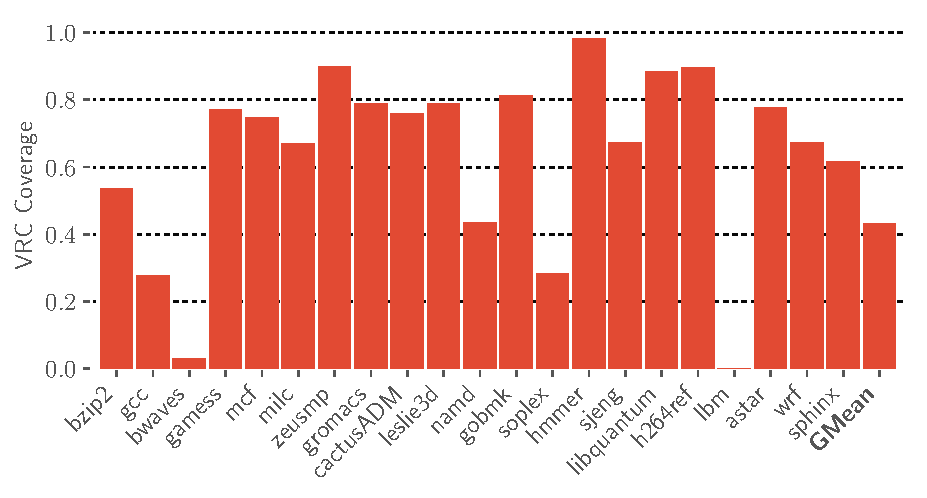
\includegraphics[width=\columnwidth]{figs/vrc_coverage.pdf}
  \caption{The coverage of the \recomp, i.e., the ratio of shadowed L1 misses that can be recomputed instead of being delayed.}
  \label{fig:rc-coverage}
\end{figure}

\begin{figure}[t]
  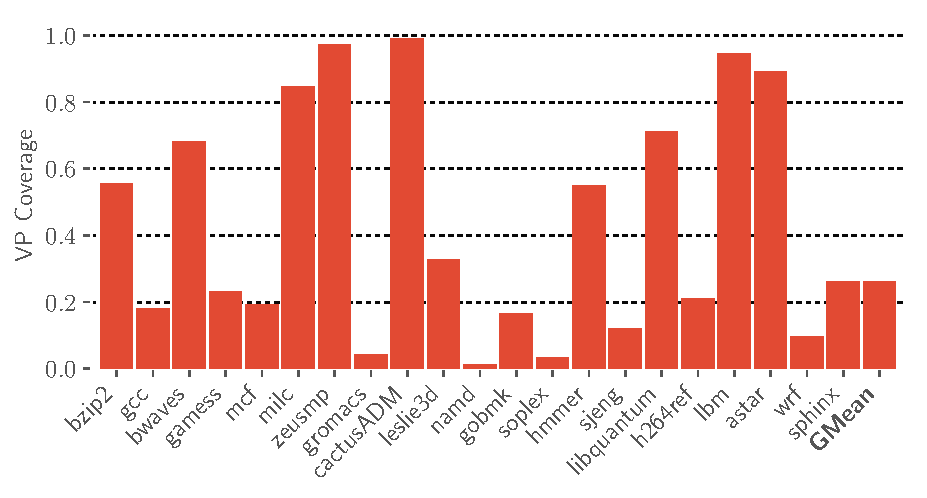
\includegraphics[width=\columnwidth]{figs/vp_coverage.pdf}
  \caption{The coverage of the VP, i.e., the ratio of shadowed L1 misses that can be predicted instead of being delayed.}
  \label{fig:vp-coverage}
\end{figure}
}

\begin{figure}[t]
  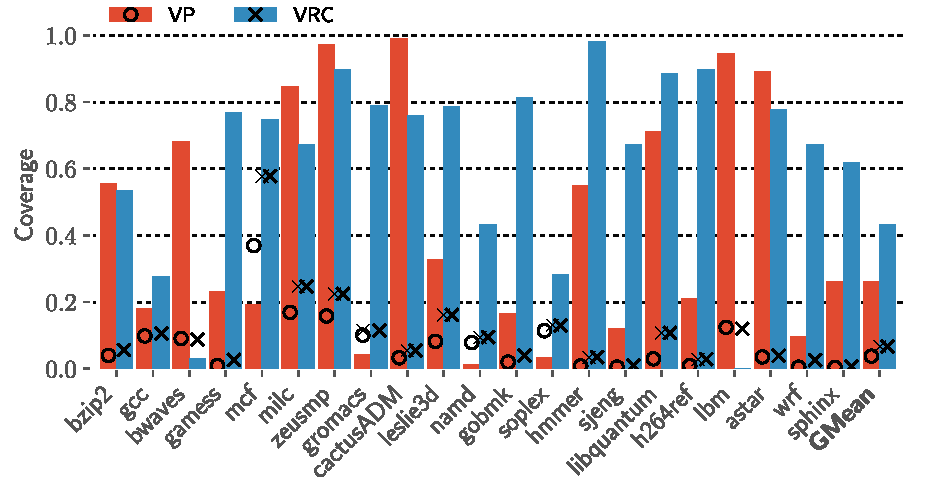
\includegraphics[width=\columnwidth]{figs/coverage.pdf}
  \caption{The coverage of the VP and the \recomp, i.e., the ratio of shadowed L1 misses that can be recomputed instead of being delayed (bars). Also on the same plot, the L1 miss ratio for both versions can be seen (circles/crosses).}
  \label{fig:coverage}
\end{figure}

\begin{figure}[t]
  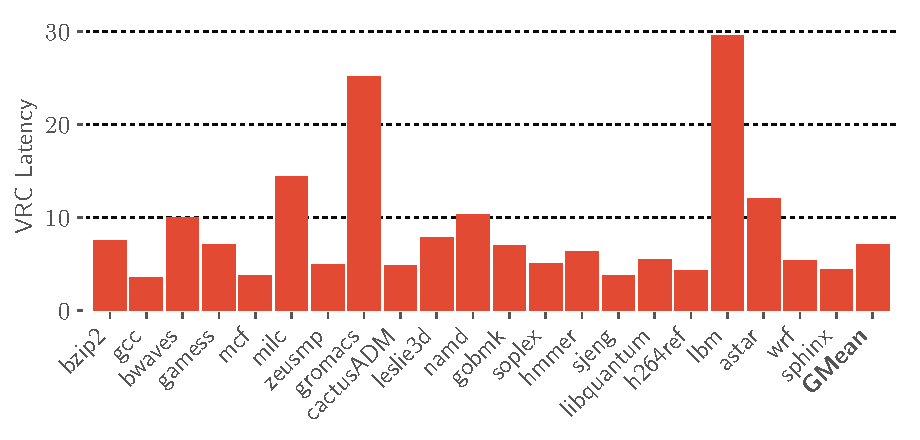
\includegraphics[width=\columnwidth]{figs/vrc_latency.pdf}
  \caption{The mean latency for recomputing a shadowed L1 miss.}
  \label{fig:rc-latency}
\end{figure}

\begin{figure*}[t]
  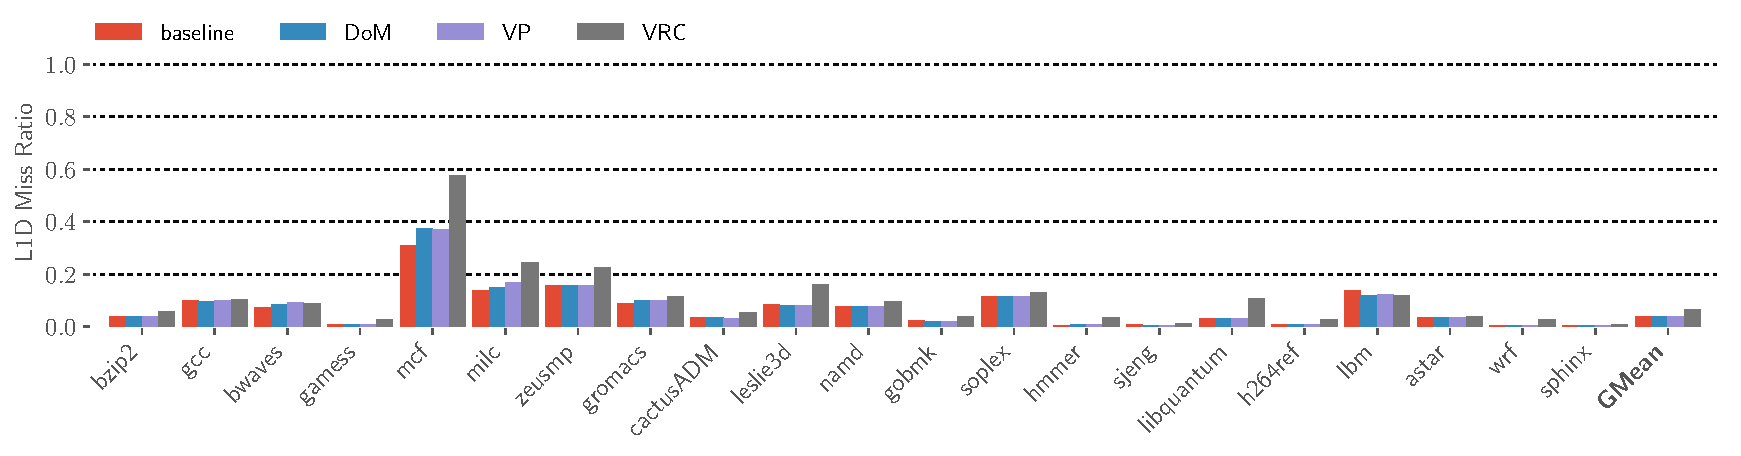
\includegraphics[width=\textwidth]{figs/l1d_miss_ratio.pdf}
  \caption{L1D miss ratio for Delay-on-Miss with VR and \recomp.}
  \label{fig:l1d_misses}
\end{figure*}

\begin{figure*}[t]
  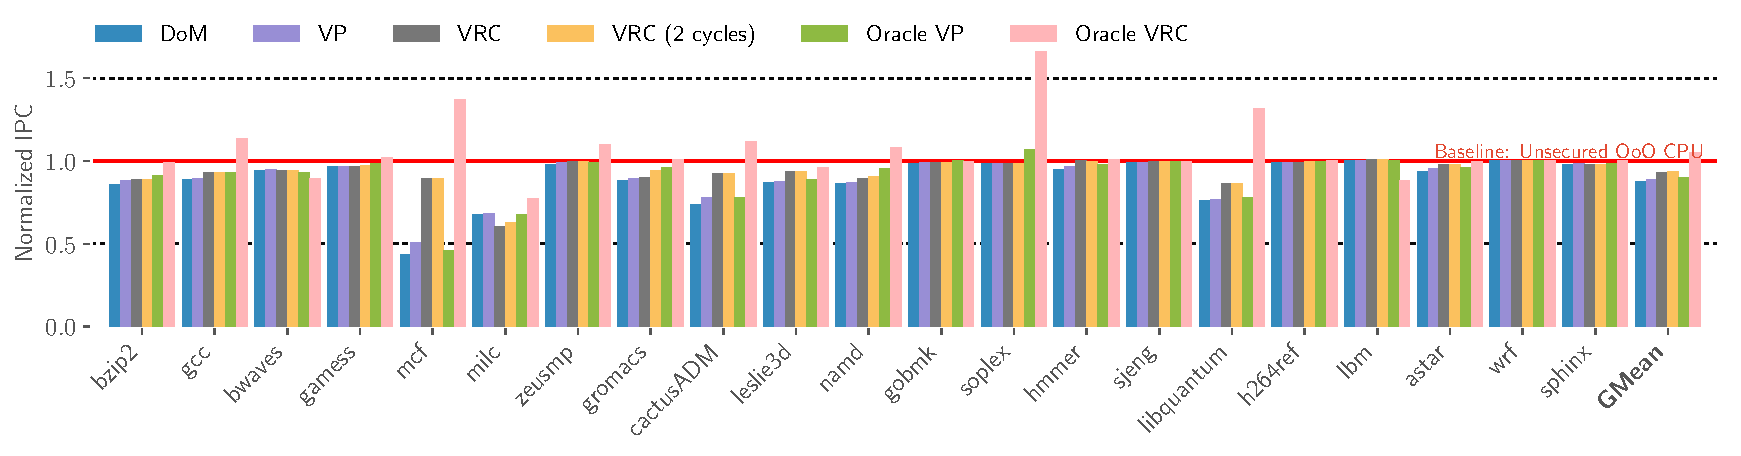
\includegraphics[width=\textwidth]{figs/normalized_ipc_all.pdf}
  \caption{Performance (IPC -- higher is better) normalized to an unsecured OoO baseline.}
  \label{fig:ipc}
\end{figure*}


\begin{figure*}[t]
  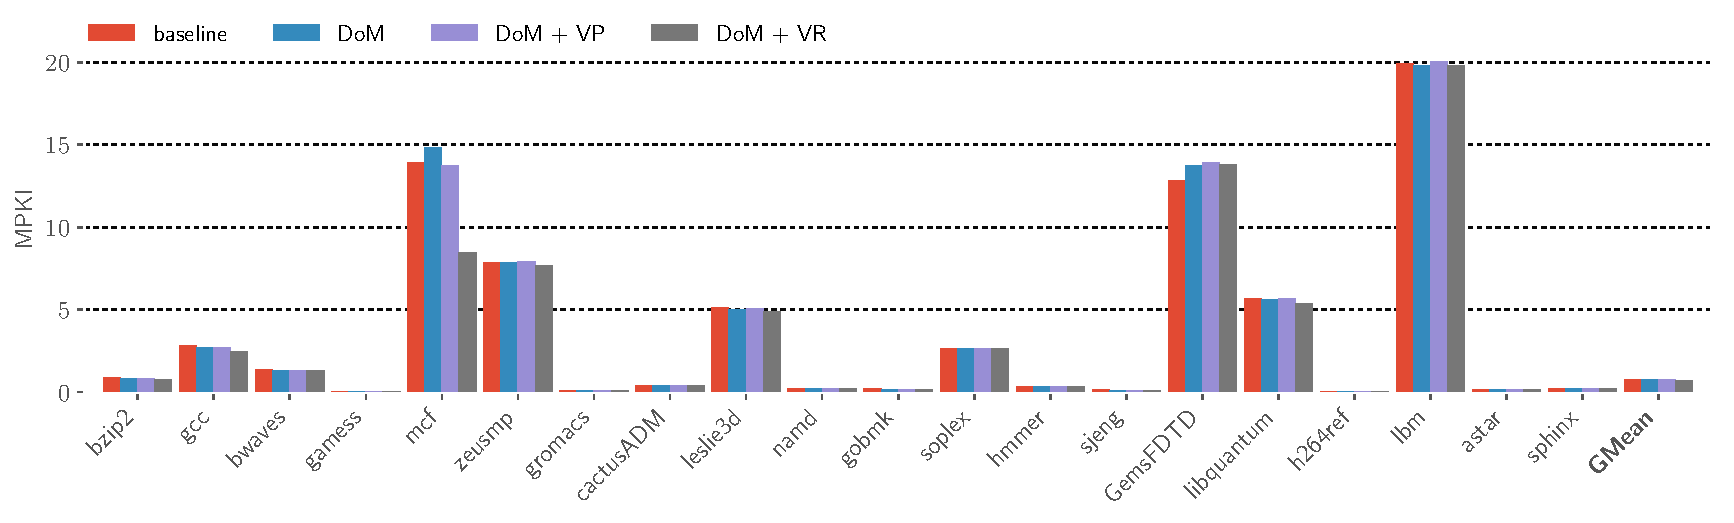
\includegraphics[width=\textwidth]{figs/mpki.pdf}
  \caption{LLC misses per 1000 instructions (MPKI).}
  \label{fig:mpki}
\end{figure*}

\begin{figure*}[t]
  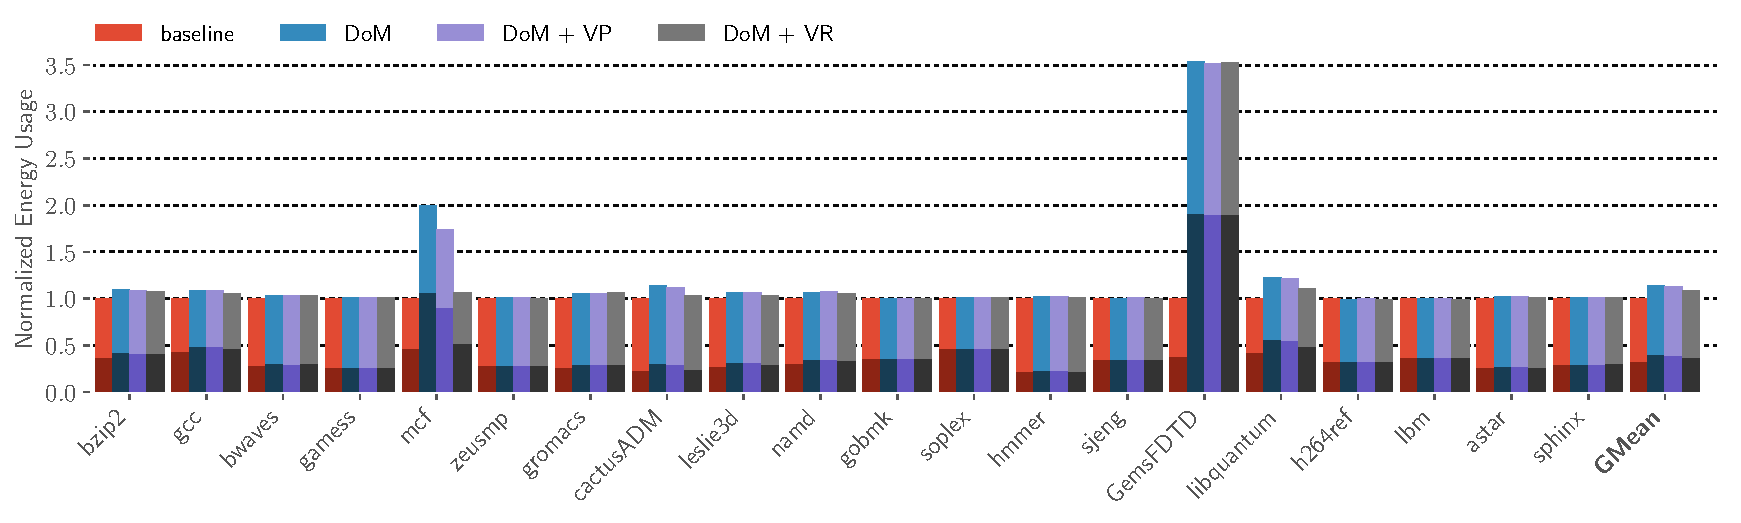
\includegraphics[width=\textwidth]{figs/normalized_energy_usage.pdf}
  \caption{Energy usage, where each bar consists of four parts (from bottom up): The bottom, light colored part is the dynamic energy of the CPU, the middle, dark colored one is the static energy of the CPU, the middle light part is the DRAM energy, including refresh and power-down energy, and the top dark part is the overhead of VP and VRC, both static and dynamic.
  }
  \label{fig:energy}
\end{figure*}

%\redHL{We should have a couple of lines of text here, between the section header and the subsection.}

\subsection{Recomputation Coverage}
\label{sec:coverage}

The coverage for the {\recomp} can be seen in \autoref{fig:coverage}, together with the VP coverage. We can immediately observe that, on average, VRC has higher coverage than VP, at $43\%$ of all speculative L1 misses vs $26\%$ with the VP. A notable example is \texttt{mcf}, which is one of the worst performing benchmarks with DoM (\autoref{sec:performance}). On the other hand, \texttt{lbm} is a counter-example, where we have almost zero VRC coverage. This, however, does not affect the performance negatively, as \texttt{lbm} does not suffer from any performance penalties even with the plain DoM.

On the same figure we have also superimposed the cache miss ratio for both versions. We only predict or recompute L1 misses, so the miss ratio is needed in conjunction with the coverage to infer the percentage of loads in the application that are being predicted or recomputed. More detailed L1D miss data can be found in \autoref{fig:l1d_misses}. Note how, as discussed in~\autoref{sec:limitations}, \recomp{} increases the miss ratio.

With VP, all loads that can be predicted are predicted in the same amount of time (2 cycles in our setup), but the same is not true for the VRC, where the latency depends on the slice length and the instructions it contains. In \autoref{fig:rc-latency} we can see the mean recomputation latency for each benchmark, as well as the overall mean. In all cases, VRC requires more cycles than VP to recompute a value, with a mean of seven cycles per slice. However, as we will see in~\autoref{sec:performance}, this does not impact the performance significantly.

\subsection{Performance}
\label{sec:performance}

\autoref{fig:ipc} contains the number of committed instructions per cycle, normalized to the unsecured baseline processor. 
Delay-on-Miss without VP or \recomp, which is our \emph{secure} baseline, performs at $88\%$ of the unsecured baseline, similarly to the results reported by Sakalis et al~\cite{sakalis+:ISCA2019vp}. 
%The two benchmarks that incur the biggest hit in performance are \texttt{GemsFDTD} (at $20\%$ of the baseline) and \texttt{mcf} ($44\%$), followed by \texttt{cactusADM} ($74\%$) and \texttt{libquantum} ($76\%$). 
The benchmarks that incurs the biggest hit in performance is \texttt{mcf} (at $44\%$ of the baseline), followed by \texttt{milc} ($68\%$), \texttt{cactusADM} ($74\%$) and \texttt{libquantum} ($76\%$).
Out of these benchmarks, three (\texttt{mcf}, \texttt{milc}, and \texttt{libquantum}) have high LLC MPKI (\autoref{fig:mpki}), but that in itself is not the only factor, as other benchmarks (e.g., \texttt{lbm}) also have a high MPKI. 
Instead, the cost of Delay-on-Miss also depends on the amount of MLP that the benchmarks exhibit; the more MLP that is taken advantage of in the baseline, the higher the performance loss. 
%This is particularly true for \texttt{GemsFDTD}, which is one of the benchmarks with a large number of concurrent long latency loads to multiple cache lines.

If VP is introduced, then the performance is similar, at $89\%$ of the unsecured baseline.
This result contradicts the results given by Sakalis et al.~\cite{sakalis+:ISCA2019vp}, where the VP gives a significant performance advantage\footnote{We contacted the authors and verified that our results are indeed valid.}. %TODO: This should be rewritten when we are no longer anonymous
The reason that VP does not offer a significant advantage is because VP itself is speculative: When a value is predicted it still needs to be validated at a later point. 
By predicting the value, a small amount of parallelism (ILP) can be exploited during execution, but the slow L1 misses still need to be satisfied for the validation. 
Due to the high number of speculative shadows, validations becomes serialized and are not able to take advantage of any MLP that might be found in the application. 
In essence, the VP pushes the cost of delaying speculative loads from the execution stage to the validation stage, but it does not eliminate it. 
This can be seen in the Oracle VP results, where even $100\%$ prediction rate (i.e., all shadowed L1 misses are successfully predicted) only leads to a marginal performance improvement of one percentage point.

The same is not true for \recomp, as once a value has been recomputed, it does not need to be validated, meaning that the cost for delaying a long latency miss is eliminated and no  serialization is enforced.
While \recomp{} does not increase the amount of MLP that can be taken advantage of, it does eliminate some of the need for it.
Overall, \recomp{} performs at $93\%$ of the unsecured baseline, decreasing the performance cost of Delay-on-Miss by more than one third (specifically, by $42\%$).
The benchmark with the most dramatic performance increase is \texttt{mcf}, which is the worst performing benchmark for Delay-on-Miss. 
\recomp{} improves the performance from $44\%$ to $90\%$, reducing the performance cost to one fifth of that of Delay-on-Miss. 
%\redHL{Unfortunately, in the case of \texttt{GemsFDTD} (the worst performing benchmark), we have a very low slice coverage, meaning that most of the loads cannot be recomputed.} 
%Because of this, \recomp, much like VP, does not improve the performance over Delay-on-Miss.

We have also evaluated an artificial version of \recomp{} where we keep the same slice coverage but reduce the cost of the slices to at most two cycles. This version exhibits almost identical performance to the real \recomp{}, with a mean performance difference of half a percentage point. This strongly indicates that instead of trying to keep the cost of the slices low, it is more important to increase the coverage, even if large slices are required. This is further corroborated by the results from the Oracle version, discussed below. However, large slices do increase the energy usage, as we will see in ~\autoref{sec:energy}, so a balance still needs to be kept.

If we introduce an Oracle \recomp{} that can recompute all shadowed L1 misses, the difference between the VP and the \recomp{} approaches becomes even more apparent. 
Both Oracle versions have $100\%$ coverage and the same latency, the only difference is that with VP the loads need to be validated when they are unshadowed, while with \recomp{} they are completed as soon as the value has been recomputed.
While, as we have seen, the VP Oracle can only achieve marginal improvements over the non-Oracle version, the \recomp{} Oracle is able to outperform even the baseline, including benchmarks such as \texttt{mcf}, \texttt{cactusADM}, and \texttt{libquantum}.
Of course, such an Oracle is unrealistic, but it does support our argument that the limiting factor for VP is the cost of validation.
%Additionally, given the $3.5\times$ over the baseline performance improvement we can observe in \texttt{GemsFDTD}, it further validates our analysis that \texttt{GemsFDTD} suffers from a lot of long latency misses that require a lot of MLP to hide.}


However, it is worth noting here that a 100\%-coverage {\recomp} does not necessarily guarantee that the performance will exceed that of the baseline. In fact, there are four benchmarks where the Oracle VRC is slower than the baseline: \texttt{bwaves}, \texttt{milc}, \texttt{leslie3d}, and \texttt{lbm}. Out of these, the \texttt{bwaves} and \texttt{lbm} {\recomp} Oracle is also slower than DoM.
There are various factors that contribute to this result: In \texttt{bwaves} and \texttt{leslie3d} the L1 and the L2 miss ratio (not shown) is increased significantly with the Oracle; in \texttt{milc} the Oracle increases the number of write misses in the L1 (not shown), as well as the average write miss latency (not shown); finally in \texttt{lbm} a combination of many factors contribute to worse cache performance.
The problem is that, even with $100\%$ coverage, not every single memory access is recomputed: Stores, non-speculative loads, and speculative L1 misses that hit in the MSHRs, are still served by the memory hierarchy. By recomputing the rest of the loads, which account for the majority of the L1 misses, the Oracle \recomp{} disrupts the normal operation of the cache and the prefetcher, resulting in performance losses. Essentially, there is a trade-off between the benefits of eliminating long-latency L1 misses and the cost of disrupting the normal cache operation.
For the majority of the benchmarks, this trade-off leans towards the benefits, but this is not true for all of the benchmarks.
Future work aiming to increase {\recomp} coverage must account for these factors to achieve optimal performance.
%I believe that the reason for the performance cost is disrupting the cache. For the paper, I am not 100\% convinced I can explain all of them in detail, so I suggest going with the more generic approach: VRC disrupts the cache, which causes performance loss, and there is a trade-off between this loss and the gain from recomputation.



\subsection{Energy Efficiency}
\label{sec:energy}

Energy efficiency, in our case, is affected by three main factors: The execution time/performance, the number of accesses in the memory hierarchy (especially the DRAM), and the cost of predicting (VP) or recomputing (VRC) a value.
\autoref{fig:energy} shows, starting from the bottom, the dynamic (bottom, light color) and static (middle, dark color) energy of the CPU, the total DRAM energy (middle, light), and, finally, the overhead (if any) for VP and VRC (top, dark). %
Overall Delay-on-Miss and VP increase the mean energy usage over the unsecured baseline by $6\%$, while \recomp{} increases it by $5\%$. The dynamic energy of the CPU (excluding the overheads) remains mostly the same across all versions, instead it is the static, DRAM, and overhead energy that changes.

Static energy is affected because the execution time is affected. This is most obvious in \texttt{mcf}, the application with the worse DoM performance, followed by \texttt{milc}. As can be seen in~\autoref{fig:mpki}, none of the evaluated solutions affect the MPKI significantly, so the increase in the DRAM energy is not due to an increase in the number of accesses but due to other operations such as refresh and power-down states. These operations do depend on the access patterns, but they also depend on the execution time, similar to the static energy usage of the system.

On the other hand, the overheads introduced by the VP and the \recomp{} are affected both by the execution time (static energy) and by the operations performed. This is particularly visible in the case of the \recomp{}, where the majority of the overhead is due to the instructions of the slices. As we have discussed in ~\autoref{sec:performance}, smaller slices do not lead to better performance, but the same is not true for the energy costs. Instead, a balance between coverage (which increases the performance) and slice length (which increases the energy usage) needs to be achieved, but such an exploratory study is beyond the scope of this work and is left as future work.

Out of all the benchmarks, the ones with the highest (relative to the baseline) energy usage are \texttt{milc} (at $37\%$ over the baseline), \texttt{gromacs} ($13\%$) and \texttt{libquantum} ($12\%$). The rest of the benchmarks have energy overheads of less than $10\%$ over the baseline. \texttt{milc} is the benchmark with the worse performance, so part of the energy increase is due to static and DRAM energy. It also has a high \recomp{} coverage and also some of the third most expensive (in cycles, on average) slices among all the benchmarks, which increases the \recomp{} overhead energy. On the other hand, \texttt{gromacs}'s performance comes very close to the baseline, but it does have the second most expensive slices, while also having high coverage. Finally, \texttt{libquantum} also sees an increase in execution time and by extension, energy usage. The next benchmark with the higher energy increase over the baseline is \texttt{mcf} ($9\%$), but this is far better than DoM, with or without VP, which is at $63\%$ and $84\%$ respectively.

%\texttt{GemsFDTD} and \texttt{mcf} incur a $3.5\times$ and $2\times$ performance overhead respectively. 
%As previously discussed in the performance analysis (\autoref{sec:performance}), \recomp{} does not improve the results for \texttt{GemsFDTD} due to low coverage, but it does decrease the overhead for \texttt{mcf} to just $6\%$ over the baseline. 
%This is a combination of both reducing the execution time and reducing the MPKI/DRAM accesses. 
%In contrast, the VP incurs an overhead of $1.7\times$ over the baseline.

%\subsection{Memory Behavior}
%\label{sec:memory}

\section{Related Work}
\label{sec:rel}
\ignore{
{\color{red} Stefanos: I've got this}
\begin{verbatim}
    1 Making speculation "invisible"
      Can we come up w/ a taxonomy?
        Coverage, complexity, ...?
    2 Cache side channels 
        [Omit?]
    3 Other related work?
        [Omit?]
\end{verbatim}
}

%\paragraph{First response techniques: delay, hide\&replay, or cleanup?}
%\paragraph
%\noindent \textbf{First response techniques: delay, hide\&replay, or cleanup?}
The architecture community promptly proposed a number of techniques (starting with the ground-braking \emph{InvisiSpec} work~\cite{yan_invisispec:MICRO2018}) to prevent \emph{disclosure gadgets} from revealing secrets. 
The techniques fall in one of the following three broad categories shown below but each individual proposal has different assumptions as to the threat model (type of speculation shadows covered) and prevention of information leakage (disclosure gadgets). 
It is obvious that at this point no direct comparison is possible but we make an effort to compare the solutions qualitatively.

%\squishlist
\textbf{Hide\&Replay:} Perform speculative memory accesses in a manner that does not perturb any $\mu$--architectural state in the memory system;
%(except DRAM row buffers which is unavoidable {\color{blue}CS: What about closed-page row buffers, as some works claim? Maybe we should avoid talking about DRAM here}); 
subsequently, perform a replay of the access (when it becomes non-speculative) to affect the correct changes in the $\mu$-architectural state. \emph{Invisispec} (Yan et al.)~\cite{yan_invisispec:MICRO2018} and \emph{Ghost loads} (Sakalis et al.)~\cite{sakalis+:CF2019ghost} were the first such proposals. 
Hide\&Replay techniques, as the first to be proposed, showed a significant cost in performance (and a moderate implementation cost). They only protect against information leaks via the memory hierarchy (and not even all of it, as DRAM leaks are possible~\cite{pessl2016drama}). On the other hand, both of these techniques were designed to protect against attacks on any possible speculation primitive, i.e., cover all the speculative shadows mentioned above. 

\textbf{Delay:} Delay speculative changes in $\mu$-architectural state until execution is non-speculative. Sakalis et al. proposed to delay loads that miss in the L1 (\emph{Delay-on-Miss}) until they are non-speculative~\cite{sakalis+:ISCA2019vp}. This delays any $\mu$-state change in the memory hierarchy. A different form of delay (\emph{NDA}) proposed by Weisse et al., is to prevent speculative data propagation by delaying \emph{dependent instructions} from executing with speculative inputs~\cite{weisse2019nda, yu_speculative:MICRO2019-STT, fustos+:DAC2019spectreguard}. Delay-on-Miss protects against \emph{all} speculative shadows (i.e., any possible ``Speculation Primitive'') but delays only changes in the memory hierarchy (including DRAM). Subsequent work, that delays speculative propagation of data~\cite{weisse2019nda}, achieves good performance by protecting against any $\mu$-architectural state changes (i.e., a much larger gamut of ``disclosure gadgets'' than just the memory hierarchy) but responding only to C-Shadows, i.e., control speculation primitives.

\textbf{Cleanup:} Perform a speculative change in $\mu$-architectural state but then \emph{undo} if speculation is squashed. In the first such proposal, \emph{CleanupSpec}, by Sailshwar et al.~\cite{saileshwar2019cleanupspec}, the undo is expensive so its application is restricted to the L1 cache. The rest of the memory hierarchy (L2, LLC, and coherence Directory) is assumed to be protected in other ways, including randomization and delaying of coherence state changes, but DRAM row buffers still remain a security hole.
Cleanup techniques only protect the L1, assuming---at a cost---that the rest of the hierarchy (excluding DRAM) is protected otherwise~\cite{saileshwar2019cleanupspec}.


\textbf{(Generic) Recomputation:} Amnesiac~\cite{amnesiac17} introduces a microarchitecture for recomputation that differs from \arch{} in the way slices are generated and their usage.
%There is a semantic difference between Amnesica and \arch\ that reveals itself in slice generation and its usage.
%There is a fundamental difference in \rs\ generation and its usage. 
%\arch\ diverges from Amnesiac when it comes to baking {\rs}s into the binary, as well:
The goal of Amnesiac is to replace as many energy-hungry loads as possible with backward slices that recompute the respective data value. % (which otherwise would be loaded from the memory hierarchy). 
%In this case, the swapped load instructions are never performed (i.e., slices in~\cite{amnesiac17} are for values corresponding to loads). 
%However, as opposed to~\cite{amnesiac17}
In contrast, ISER recomputes slices selectively, such that recomputation is triggered only for shadowed loads that miss in L1.

Kandemir et al., proposed a recomputation-based approach to reduce off-chip memory space in embedded processors~\cite{Kandemir:2005gw}.  
Koc et al. investigated how recomputation of data residing in memory banks in low-power states can reduce the energy consumption~\cite{Koc:2006ce}, and devised compiler optimizations for scratchpads~\cite{Koc:2007bl} that are limited to array variables.
The dual of recomputation, \emph{memoization}~\cite{Sodani:1997hn, resistiveComp} replaces computation with table look-ups for pre-computed values (for the ones that are frequent and expensive to recompute). Memoization can mitigate the communication overhead, since table
look-ups are much cheaper than long-distance data retrieval. 
Memoization is only effective if the respective computations exhibit significant value locality. 
Therefore, memoization and recomputation can complement each other in boosting energy efficiency.
\emph{Idempotent Processors}~\cite{idem} execute programs as a sequence of
compiler-constructed idempotent (i.e., re-executable without any side effects) code regions.  
As the name suggests, idempotent regions regenerate the same output regardless of how many times they are executed with the given program state.  
Generally, idempotent regions are larger, and therefore tend to incur higher overhead for recomputation, while slices for VRC employ fine-grained data recomputation (along a short, independent slices for each value), where each slice contains only the necessary instructions to generate a value. 
Accordingly, slices for VRC may provide more flexibility than idempotent regions.

Elnawawy et al., demonstrated the applicability of recomputation to loop-based
code~\cite{Elnawawy2017} to reduce checkpointing overheads. 
In their proposal, a whole
loop is (re)executed during recovery, where only the initial state of the loop is
required to be checkpointed. 
The loops may contain extra computations that
are not relevant to the production of the value to be recovered. 
Compared to such a coarse-grain recomputation,
slice-based recomputation does not contain any irrelevant instructions. Also, slices used for VRC do not contain load
instructions, as opposed to~\cite{Elnawawy2017}; and recomputation applies outside of loops provides a wider applicability.
Although value recomputation has been explored in different contexts before, to the best of our knowledge, none of the prior works have evaluated recomputation in the context of security.


\section{Conclusion}
\label{sec:conc}
\ignore{
\begin{verbatim}
    Summary
        Problem, solution, evaluation
    Discuss 
        Coverage
        Limitations
        New vulnerabilities? 
\end{verbatim}
}
\emph{Delay} techniques aim to hide the effects of transient execution by simply delaying instructions until they become non-speculative. Whether delaying loads that miss in the L1, as Delay-on-miss does, or delaying the propagation of speculative data to dependent instructions, as NDA and STT do, delay techniques extract a heavy toll in performance, in direct relation to the set of speculation shadows they protect. Delay techniques would be at an impasse with respect to improvement if we could not regain some of this lost performance in some other way. To this end, value prediction, invisible from the outside, was initially proposed as a solution.

In this work, we show that value prediction is not the right abstraction for recovering lost performance in Delay-on-miss. This is not because of coverage or accuracy but because value prediction is just another form of speculation that needs to be validated. Validation limits the potential benefits to the point where even an oracle VP (100\% coverage and accuracy) does not do any better than a practical VP. In our evaluation we found that, no matter how good, VP is limited to just one percentage point improvement over Delay-on-miss.

Instead, we propose another, \emph{non-speculative}, abstraction to regain performance for delay techniques, and in particular for Delay-on-miss. We propose to use recomputation that yields correct values---not predictions---as the key to overcome Delay-on-miss performance limitations. We describe the architecture, we evaluate it using a practical approach to generate recomputation slices albeit with modest coverage, and we exceed the performance of Oracle VP ($90\%$ vs $93\%$) with lower energy usage. Finally, we discuss the potential for increasing the coverage of recomputation with future architectural support. Because, as we show, oracle recomputation easily exceeds even the performance of the unmodified (unsecured) baseline, this direction provides tangible motivation for researching techniques for a future secure processor. % that can exceed the performance of the baseline.





%\section*{Acknowledgements}
%\input{ack}

%%%%%%% -- PAPER CONTENT ENDS -- %%%%%%%%

%%%%%%%%% -- BIB STYLE AND FILE -- %%%%%%%%
\bibliographystyle{IEEEtranS}
\bibliography{refs}
%%%%%%%%%%%%%%%%%%%%%%%%%%%%%%%%%%%%

\end{document}

